\section{Temas de Pesquisa}

\subsection{TCC}
\begin{frame}
	\frametitle{Temas de Pesquisa - TCC}
	Simulação de redes de sensores sem fio com o Network Simulator
	\begin{itemize}
		\item Protocolos de comunicação
		\item Módulo de simulação
		\item Customização na configuração do ambiente simulado
		\item Integração com outros módulos
	\end{itemize}
\end{frame}


\subsection{Mestrado}
\begin{frame}
	\frametitle{Temas de Pesquisa - Mestrado}
	Analysing Feature Dependencies in Preprocessor-Based Systems
	
	\begin{itemize}
		\item[] 
	\end{itemize}
	
	O Problema:
	\begin{columns}
	\begin{column}{4cm}
	\begin{itemize}
		\item[]<1-> \texttt{void m()\{}
		\item[]<1-> \texttt{$\quad$...}
		\item[]<1-|alert@2-> \texttt{$\quad$int x = 0;}
		\item[]<1-> \texttt{\textbf{$\quad$\#ifdef} SQRT}
		\item[]<1-|alert@3-> \texttt{$\qquad$sqrt(x);}
		\item[]<1-> \texttt{\textbf{$\quad$\#endif}}
		\item[]<1-> \texttt{$\quad$...}
		\item[]<1-> \texttt{\}}
	\end{itemize}
	\end{column}

	\begin{column}{6cm}
		\begin{overlayarea}{\textwidth}{.4\textheight}
			\begin{onlyenv}<4>{If \texttt{\textbf{x = -1}} ?}\end{onlyenv}
		\end{overlayarea}
	\end{column}
	\end{columns}
\end{frame}

\begin{frame}
	\frametitle{Temas de Pesquisa - Mestrado}
	O estudo:
	\begin{itemize}
		\item Análise de $51$ SPLs baseadas em pré-processadores
		\item Diferentes domínios, tamanhos e linguagens (C e Java)
		\item Uso de diretivas de compilação condicional
		\item Utilização de ferramentas auxiliares
	\end{itemize}
\end{frame}

\begin{frame}
\frametitle{Temas de Pesquisa - Mestrado}
	Perguntas de Pesquisa:
	\begin{itemize}
		\item Como o tamanho do programa influencia nas dependências entre features?
		\item Como os mecanismos de variabilidade influenciam nas dependências entre features
		\item Como o número de features influencia nas dependências entre features?
	\end{itemize}
\end{frame}

\begin{frame}
	\frametitle{Temas de Pesquisa - Mestrado}
	\begin{center}
		\begin{figure}
			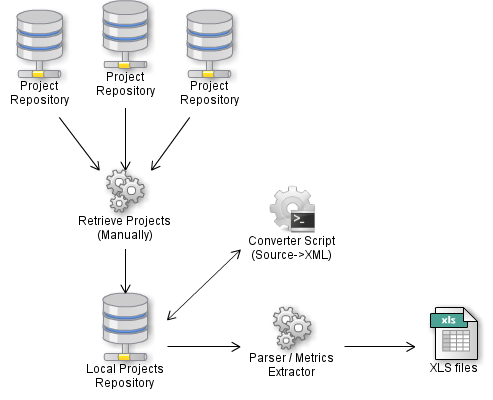
\includegraphics[width=.7\linewidth]{images/infrastructure}
		\end{figure}
	\end{center}
\end{frame}

\begin{frame}
	\frametitle{Temas de Pesquisa - Mestrado}
	Alguns números:
	\begin{itemize}
		\item $39$ projetos em C
		\item $12$ projetos em Java
		\item $56233$ arquivos convertidos
		\item $606118$ métodos analisados
		\item $23$ ($0,04\%$) arquivos excluídos
	\end{itemize}
\end{frame}

\begin{frame}
\frametitle{Temas de Pesquisa - Mestrado}
\begin{center}
	\begin{figure}
		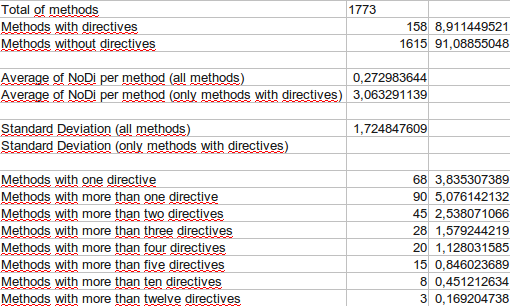
\includegraphics[width=.7\linewidth]{images/directives3}
	\end{figure}
\end{center}

\begin{center}
	\begin{figure}
		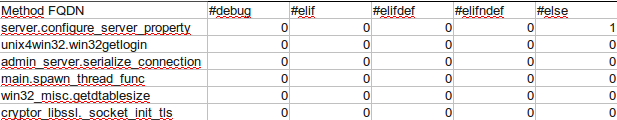
\includegraphics[width=.7\linewidth]{images/directives1}
	\end{figure}
\end{center}
\end{frame}

\begin{frame}
	\frametitle{Temas de Pesquisa - Mestrado}
	Trabalhos futuros/não realizados:
	\begin{itemize}
		\item Definição de uma maneira sistemática para realizar uma busca em repositórios de bugs
		\item Como as dependências entre features influenciam os bugs introduzidos em tarefas de manutenção de uma SPL?
		\item Criação de uma ferramenta para download automático de projetos
		\item Como analisar dependências interprocedurais?
	\end{itemize}
\end{frame}

\begin{frame}
	\frametitle{Temas de Pesquisa - Mestrado}		
	Referências:
	\begin{itemize}
		\item Facilities and pitfalls of macro expansion (Ernst et al., TSE 2002)
		\item Feature code scattering and tangling (Liebig et al., ICSE 2010)
		\item Program variability quantification (Sincero et al., GPCE 2010)
		\item Disciplined and undisciplined annotations (Liebig et al., AOSD 2011)
	\end{itemize}
\end{frame}

\subsection{Atividades Atuais}
\begin{frame}
	\frametitle{Temas de Pesquisa - Atividades Atuais}
	Análise de Sistemas: Integração/Automação de artefatos
	\begin{itemize}
		\item[]
	\end{itemize}

	Motivação/Problemas:
	\begin{itemize}
		\item Resultado da análise: documentação
		\item Boa parte da documentação serve apenas como prova de que algo foi feito, mas não é útil.
		\item Documentar é realmente necessário? 
		\item Qual o nível de detalhamento?
		\item Como prover artefatos que sejam aproveitados pelos clientes e pela equipe de desenvolvimento?
	\end{itemize}
\end{frame}

\begin{frame}
	\frametitle{Temas de Pesquisa - Atividades Atuais}
	Objetivos:
	\begin{itemize}
		\item Otimizar o conjunto de artefatos gerados
		\item Minimizar o gap entre negócio e desenvolvimento
		\item Integrar/automatizar artefatos
		\item Definir metodologias e técnicas
	\end{itemize}

	Algumas ferramentas/técnicas:
	\begin{itemize}
		\item Prototipagem - Axure, Balsamiq
		\item Automação/integração - BDD, Selenium, \LaTeX
		\item Integração contínua - Jenkins
	\end{itemize}
\end{frame}

\subsection{Outros temas de interesse}
\begin{frame}
	\frametitle{Temas de Pesquisa - Outros temas de interesse}
	Outras temas de interesse:
	\begin{itemize}
		\item Teste de Software
		\item Software livre
		\item Automação residencial
	\end{itemize}
\end{frame}
